\chapter{\textcolor{myred}{Incertidumbre de Fourier}}

\section{\huge{Motivación}}

\textcolor{myred}{\hrule}

\newthought{Imaginemos} que estamos sosteniendo el extremo de una soga, y generamos una onda sacudiéndola hacia arriba y abajo (figura \ref{fig:onda1}). Si alguien nos preguntara '¿Dónde \textit{está} exactamente la onda?' pensaríamos que la pregunta tiene muy poco sentido: la onda no está exactamente en \textit{ningún} lugar, está esparcida por unos $50m$. Por otro lado, si nos preguntara cuál es su \textit{longitud de onda}, podríamos darle una respuesta razonable, unos $6m$.
\begin{marginfigure}
\captionsetup{type=figure}
    \centering
    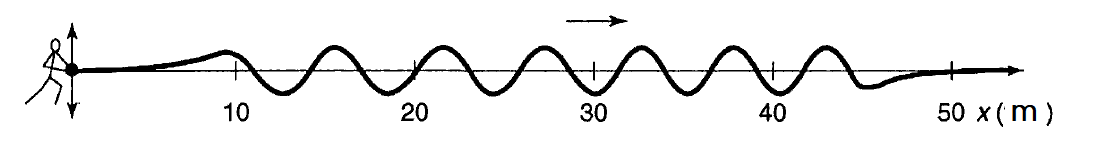
\includegraphics[width=1.3\textwidth]{Im/onda1.png}
    \caption{Una onda con \textit{longitud de onda} bastante bien definida, pero con una \textit{posición} mal definida.}
    \label{fig:onda1}
\end{marginfigure}

\begin{marginfigure}
\captionsetup{type=figure}
    \centering
    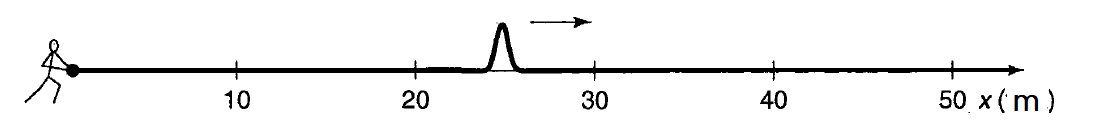
\includegraphics[width=1.3\textwidth]{Im/onda2.png}
    \caption{Una onda con \textit{posición} bastante bien definida, pero con una \textit{longitud de onda} mal definida.}
    \label{fig:onda2}
\end{marginfigure}
Si, en contraste, le diéramos una sacudida repentina a la soga, obtendríamos una perturbación delgada que viaja a lo largo de la línea (figura \ref{fig:onda2}). Esta vez la primer pregunta (¿Dónde está exactamente la onda?) es bastante razonable, y la segunda (¿Cuál es su longitud de onda?) no tiene sentido -al no parecerse a algo periódico, a priori no podemos asignarle una longitud de onda. Por su puesto, podemos plantearnos casos intermedios, en los cuales la onda esté más o menos localizada y tenga una longitud de onda más o menos definida, pero hay un intercambio inefable: cuanto más precisa sea la posición de la onda, menos precisa es su longitud de onda, y viceversa\cite[][p.30]{GriffithsCuantica}.

\vspace{0.5cm}

El propósito de este trabajo será desarrollar en profundidad este fenómeno, denominado \textbf{complementariedad}, viendo primero cómo se comportan los pares de variables $\{\omega, t\}$ y $\{k,x\}$ frente a una \textbf{transformada de Fourier}. También veremos cómo los campos reales deben representarse mediante \textbf{paquetes de ondas}, que también sufren de dicha complementariedad.
\begin{marginfigure}
\begin{qbox}{Quantum Box}
En estos recuadros vamos a mencionar el uso que tienen las definiciones y los resultados en la \textbf{mecánica cuántica}.
\end{qbox}   
\end{marginfigure}

Por último, introduciremos el concepto de \textbf{operadores} para demostrar una forma generalizada del \textbf{principio de incertidumbre}.



\newpage
\begin{intro}{}
\textbf{Comenzaremos el presente trabajo} introduciendo conceptos, extraídos de las primeras secciones del capítulo 15 del \textbf{Mathematical Methods for Physicists} (Arfken), que utilizaremos sobre Transformadas de Fourier.
\end{intro}


\section{Transformadas de Fourier}

\textcolor{myred}{\hrule}

\newthought{En física} nos encontramos frecuentemente con expresiones de la forma 
\begin{equation}
   g(\alpha) = \int_a^b f(t) K(\alpha,t) ~dt
\end{equation}
donde la función $g(\alpha)$ es la transformada (integral) de $f(t)$ mediante el kernel $K(\alpha,t)$. Esta operación se puede describir como un mapeo de la función $f(t)$ en el espacio-$t$ a otra función, $g(\alpha)$, en el espacio-$\alpha$. Esta interpretación tiene significado físico en la relación tiempo-frecuencia de las transformadas de Fourier y en la relación espacio-momento en la mecánica cuántica. 

\subsection{\textbf{Transformadas de Fourier}}
Una de las transformadas más útiles es la de Fourier, la cual esta dada por 
\begin{equation}
    \hat{f}(\omega) = \frac{1}{2\pi} \int_{-\infty}^\infty  f(t) e^{i\omega t}~dt 
     \label{gomega}
\end{equation}

Dicha transformada tiene como base el kernel $e^{i\omega t}$ dado que estos kernels son las funciones utilizadas para describir ondas planas y por lo tanto es el kernel que utilizaremos a lo largo de todo lo que sigue\footnote{Existen numerosos kenerls útiles. Por ejemplo, $e^{-\alpha t}$ para la transformada de Laplace. $tJ_n(\alpha t)$ para la transformada de Henkel y $t^{\alpha-1}$ para la transformada de Mellin.}. 

\subsection{\textbf{Integral de Fourier}}
Sabemos del estudio de las series de Fourier que \textit{si una función es periódica} podemos describirla mediante una suma de senos y cosenos. Ahora nos interesa representar funciones no periódicas en un intervalo infinito. Físicamente, esto significa describir un pulso o paquete de ondas mediante ondas sinusoidales. 

A partir de la serie de Fourier general y de los coeficientes de Fourier se puede llegar, trabajando un poco, a la integral de Fourier haciendo tender los limites de los coeficientes a $\pm \infty$ (recordar que dichos coeficientes son integrales en el intervalo $[-L,L]$). Luego la \textbf{integral de Fourier es}
\begin{equation}
    f(x) = \frac{1}{\pi} \int_0^\infty d\omega ~ \int_{-\infty}^\infty f(t) \cos{[\omega(t-x)]}~dt
\end{equation}
donde dimos por sentado que $f(x)$ es seccionalmente continua, seccionalmente diferenciable y absolutamente integrable. Se puede reescribir la integral anterior en una forma más útil y obtenemos el \textbf{teorema de la integral de Fourier}
\begin{equation}
     f(x) = \frac{1}{2\pi} \int_{-\infty}^\infty e^{-i\omega x}~ d\omega ~ \int_{-\infty}^\infty f(t) e^{i\omega t}~dt
     \label{integralfourier}
\end{equation}

Si ahora tomamos la transformada de la función $f(t)$ dada por \ref{gomega} y la reemplazamos en la integral de Fourier ec.\ref{integralfourier} obtenemos la relación inversa a la transformada, es decir, la antitransformada de Fourier
\begin{equation}
f(t)  = \int_{-\infty}^\infty \hat{f}(\omega)e^{-i\omega t}~dt 
\label{ft}
\end{equation}
el par de ecuaciones dado por \ref{gomega} y \ref{ft} constituye un \textbf{par de trasformadas de Fourier}.

Finalmente , el par de transformadas de Fourier en el espacio tridimensional es 
\begin{equation}
\begin{split}
    g(\mathbf{k}) &= \frac{1}{(2\pi)^{3/2}} \int f(\mathbf{r}) e^{i\mathbf{k}\cdot\mathbf{r}}~d^3r \\
    f(\mathbf{r}) &= \frac{1}{(2\pi)^{3/2}} \int g(\mathbf{k}) e^{-i\mathbf{k}\cdot\mathbf{r}}~d^3r
    \label{trans3d}
\end{split}    
\end{equation}
Dichas integrales son en todo el espacio, se puede verificar sustituyendo una ecuación en la otra y usando la delta de Dirac tridimensional. La segunda ecuación puede ser interpretada como la expansión de una función $f(\mathbf{r})$ en un continuo de ondas planas como funciones base donde $g(\mathbf{k})$ es la amplitud de la onda, $e^{-i\mathbf{k}\cdot\mathbf{r}}$.



\newpage
\begin{intro}{}
\textbf{Introduciremos este tema} con una aplicación simple e ilustrativa del concepto y luego entraremos más en detalle una vez introducido el concepto de paquetes de ondas.
\end{intro}
 
\section{\huge{Complementariedad}}
\textcolor{myred}{\hrule}

\newthought{Veamos la siguiente aplicación} de la transformada de Fourier. Supongamos que tenemos una tren de ondas infinito $\sin{\omega_0 t}$ recortado por una celda Kerr,\footnote{La celda de Kerr está basada en el efecto Kerr, en el cuál el nitrobenceno se vuelve birrefrigente bajo la influencia de un campo electrico. Esto permite que sea usada como obturador que puede ser abierto por un periódo muy corto de tiempo, alrededor de 10ns.} entonces tenemos
\begin{equation}
f(t)= \left\lbrace \begin{array}{lr}
\sin{\omega_0 t} \hspace{1cm} &|t| < \frac{N\pi}{\omega_0} \\
0 \hspace{1cm} &|t| > \frac{N\pi}{\omega_0}
\end{array} \right.
\end{equation}
es decir, una función que corresponde a N ciclos de nuestro tren de ondas original y luego se anula. Dado que es impar podemos utilizar la transformada de Fourier del seno\cite[][p.939]{arfken}
\begin{equation}
    g(\omega) = \sqrt{\frac{2}{\pi}} \int_0^{N\pi/\omega_0}\sin{\omega_o t} \sin{\omega t}~dt
\end{equation}
Integrando llegamos a la función para la amplitud en función de la frecuencia
\begin{marginfigure}
\captionsetup{type=figure}
    \centering
    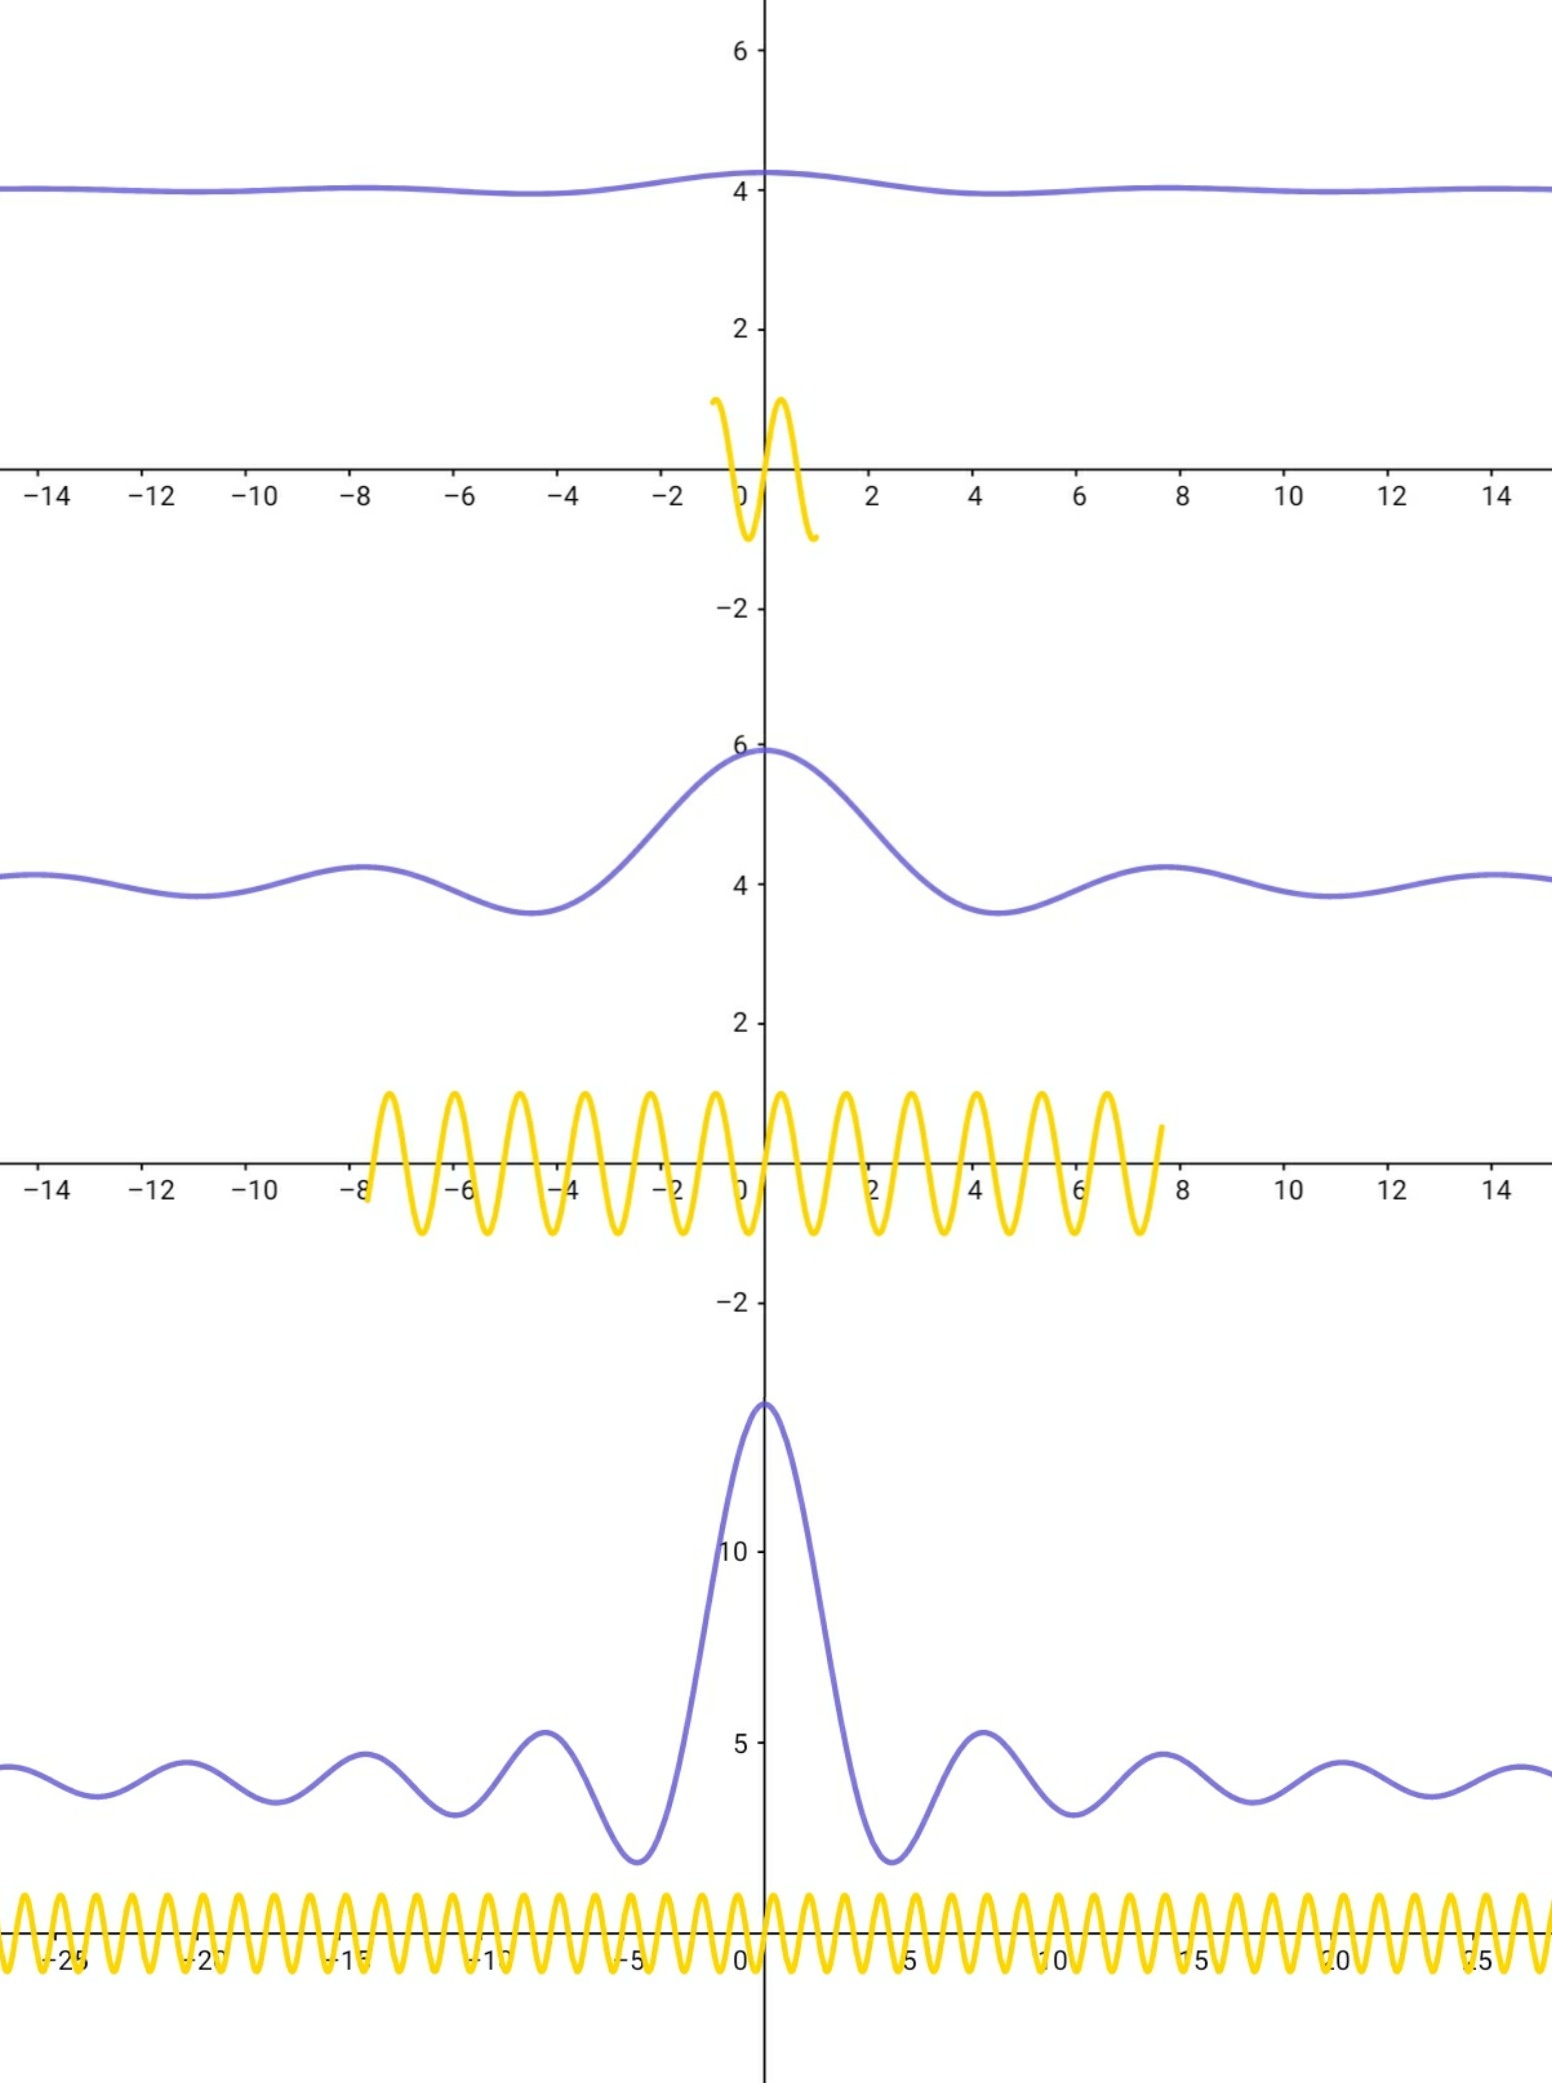
\includegraphics[width=1.3\textwidth]{Im/senoss.jpg}
    \caption{Tren de ondas (amarillo) y su respectiva transformada de Fourier (violeta), para $N=1$, $N=9$ y $N=35$}
    \label{fig:sen}
\end{marginfigure}

\begin{equation}
     g(\omega) = \sqrt{\frac{2}{\pi}}\biggr[ \frac{\sin{[(\omega_0- \omega)(N\pi/\omega_0)]}}{2(\omega_0- \omega)}-\frac{\sin{[(\omega_0+ \omega)(N\pi/\omega_0)]}}{2(\omega_0+\omega)}\biggr]
\end{equation}
Debido al denominador del primer término solo este es de importancia. Como se puede ver en la figura, esta es la curva de amplitud para el patrón de difracción de una sola rendija. Los ceros se encuentran en 
\begin{equation}
    \frac{\omega_0 - \omega}{\omega} =\frac{\Delta \omega}{\omega_0} = \pm \frac{1}{N}, ~~\pm \frac{2}{N}, ..
\end{equation}
En este caso las contribuciones fuera del ancho del máximo central son pequeñas entonces podemos restringir la dispersión en la frecuencia al primer 0 de la función como una buena medida de dicha dispersión, es decir
\begin{equation}
    \Delta \omega = \frac{\omega_0}{N}
\end{equation}

Concluimos que en este caso, si $N$ es grande (un pulso largo), la dispersión en los valores de la amplitud de la frecuencia serán pequeños. Si por el contrario, el pulso está limitado a un $N$ pequeño, la distribución de las frecuencia será mayor, y los máximos secundarios serán relevantes. Este hecho que acabamos de ver, vale para cualquier par de transformadas de Fourier y se denomina \textbf{complementariedad} y lo desarrollaremos más en profundidad en la siguiente sección

\newpage
\begin{intro}{}
\textbf{Para formalizar el concepto} enunciado en el ejemplo anterior, enunciaremos los puntos claves de las secciones 16.5.2 y 16.5.3  del \textbf{Modern Electrodynamics} (Zanguill) referida a los \textbf{paquetes de ondas escalares}.
\end{intro}

\section{\huge{Paquetes de onda}}

\textcolor{myred}{\hrule}

\newthought{Una onda plana monocromática} tiene campos que llenan todo el espacio, y energía infinita, y por lo tanto es una idealización que no puede existir en la naturaleza. Lo que sucede en realidad es que los campos, de extensión finita, forman un \textbf{paquete de ondas}, es decir, una superposición de ondas planas monocromáticas. Como las ecuaciones básicas son lineales, podemos realizar en principio superposiciones lineales de ondas planas monocromáticas con diversas frecuencias\cite[][p.323]{Jackson}. Tomaremos dichas ondas planas como \textbf{funciones base} y usaremos herramientas del \textbf{análisis de Fourier} para escribir estos campos como:
\begin{marginfigure}
\captionsetup{type=figure}
    \centering
    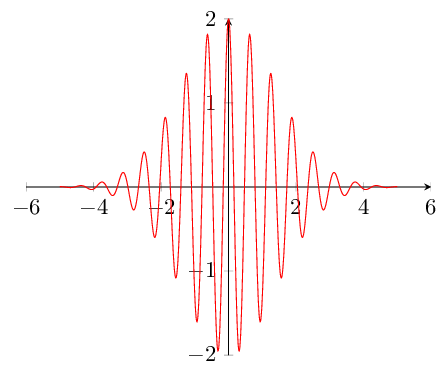
\includegraphics[width=1.3\textwidth]{Im/eoUPl.png}
    \caption{Un paquete de ondas unidimensional. Una envolvente Gaussiana de ancho $\Delta x$ modula la amplitud de una onda con vector de onda $k_{0x}$.}
    \label{fig:paquete}
\end{marginfigure}
\begin{equation}
    \mathbf{E}(\mathbf{r},t)=Re\frac{1}{(2\pi)^3}\int d^3k \, \boldsymbol{\mathcal{E}}_{\perp}(\mathbf{k})\, e^{i(\mathbf{k}\cdot \mathbf{r}-ckt)}
\end{equation}

y

\begin{equation}
    c\mathbf{B}(\mathbf{r},t)=Re\frac{1}{(2\pi)^3}\int d^3k \, \left[\boldsymbol{\hat{\mathbf{k}}\times \mathcal{E}}_{\perp}(\mathbf{k})\right]\, e^{i(\mathbf{k}\cdot \mathbf{r}-ckt)}
\end{equation}
 
Siempre que estas integrales converjan, estaremos trabajando con campos físicos asociados a un paquete de ondas.

Sabemos que es más fácil trabajar con magnitudes escalares que vectoriales, sin pérdida de generalidad, si dejamos a un lado los paquetes de onda vectoriales y comenzamos a utilizar los paquetes de onda escalares formados por suma de las soluciones de la \textbf{ecuación de onda escalar}\footnote{Se puede encontrar en las sec. 16.2.1 y 16.2.2 del Zanguill el método para generar soluciones de las ecuaciones de Maxwell en el vacío mediante el uso de potenciales electromagnéticos a partir de soluciones de la ecuación de onda escalar.} 
\begin{equation}
    \nabla^2u - \frac{1}{c^2} \frac{\partial^2 u}{\partial t^2} =0
\end{equation}

Un paquete compuesto por ondas planas monocromáticas con frecuencia $\omega(\mathbf{k})= c|\mathbf{k}|$ esta dado por
\begin{equation}
    u(\mathbf{r},t)=\frac{1}{(2\pi)^3} \int d^3~ \hat{u}(\mathbf{k}) \mathrm{exp}(i[\mathbf{k}\cdot\mathbf{r}-\omega(\mathbf{k})t])
\end{equation}

Sabemos del análisis de Fourier que la amplitud dada por $\hat{u}(\mathbf{k})$ está determinada por la forma inicial del paquete de onda\footnote{Recordar el cálculo del movimiento de una cuerda en el tiempo y en el espacio a partir de su forma inicial.} en $t=0$. De hecho, si tomamos $\hat{u}(\mathbf{k})$ y $u(\mathbf{r},0)$, comparando con \ref{trans3d} vemos que son efectivamente pares de transformadas de Fourier
\begin{equation}
    \begin{split}
        u(\mathbf{r},0) &= \frac{1}{(2\pi)^3} \int d^3k~ \hat{u}(\mathbf{k}) \mathrm{exp}(i\mathbf{k}\cdot\mathbf{r}) \\
        \hat{u}(\mathbf{k}) &= \int d^3 r ~ u(\mathbf{r},0) \mathrm{exp}(-i\mathbf{k}\cdot\mathbf{r})
    \end{split}
\end{equation}
Pasemos a un plano unidimensional tomando que las amplitudes $\hat{u}(\mathbf{k})$ solo sean no nulas en el eje $x$, es decir trabajamos solo con vectores en dicho eje, luego tenemos
\begin{equation}
     u(x,0) = \frac{1}{(2\pi)^3} dk_x~ \int \hat{u}(k_x) \mathrm{exp}(i k_x r)
     \label{transgaussiana}
\end{equation}
Ahora si elegimos que $\hat{u}(k_x)$ sea una \textbf{Gaussiana normalizada} con ancho medio $\Delta k_x$ centrada en $k_{0x}$ es decir:

\begin{marginfigure}
\begin{qbox}{}
En cuántica, los paquetes de ondas con la menor 'incertidumbre' asociada son los de forma Gaussiana.   
\end{qbox}

\end{marginfigure}

\begin{equation}
    \hat{u}(k_x) = \frac{1}{\sqrt{\pi}\Delta k_x} \mathrm{exp}\biggr[\frac{-(k_x-k_{0x})^2}{\Delta k_x^2}\biggr]
    \label{gaussiana}
\end{equation}
Calculemos entonces la transformada de Fourier de $\hat{u}(k_x)$ metiendo \ref{gaussiana} en \ref{transgaussiana} y resolviendo la integral\footnote{La siguiente integral es útil: $$\int_{-\infty}^{\infty} ds~ \mathrm{exp}(as-bs^2) = \sqrt{\frac{\pi}{b}}\mathrm{exp}(\frac{a^2}{4b})$$} llegamos a otra Gaussiana de ancho medio $\Delta x = \frac{2}{\Delta k_x}$
\begin{equation}
    u(x,0) =  \mathrm{exp}(ik_{0x}x) \mathrm{exp}\biggr[\frac{-x^2}{(\Delta x^2)^2}\biggr]
\end{equation}

Tomando la parte real de la ecuación anterior, tenemos un paquete de ondas estacionario con longitud de onda $2\pi/k_{0x}$ y amplitud modulada por una Gaussiana como se muestra en la figura \ref{fig:gau}. 
\begin{marginfigure}
\captionsetup{type=figure}
    \centering
    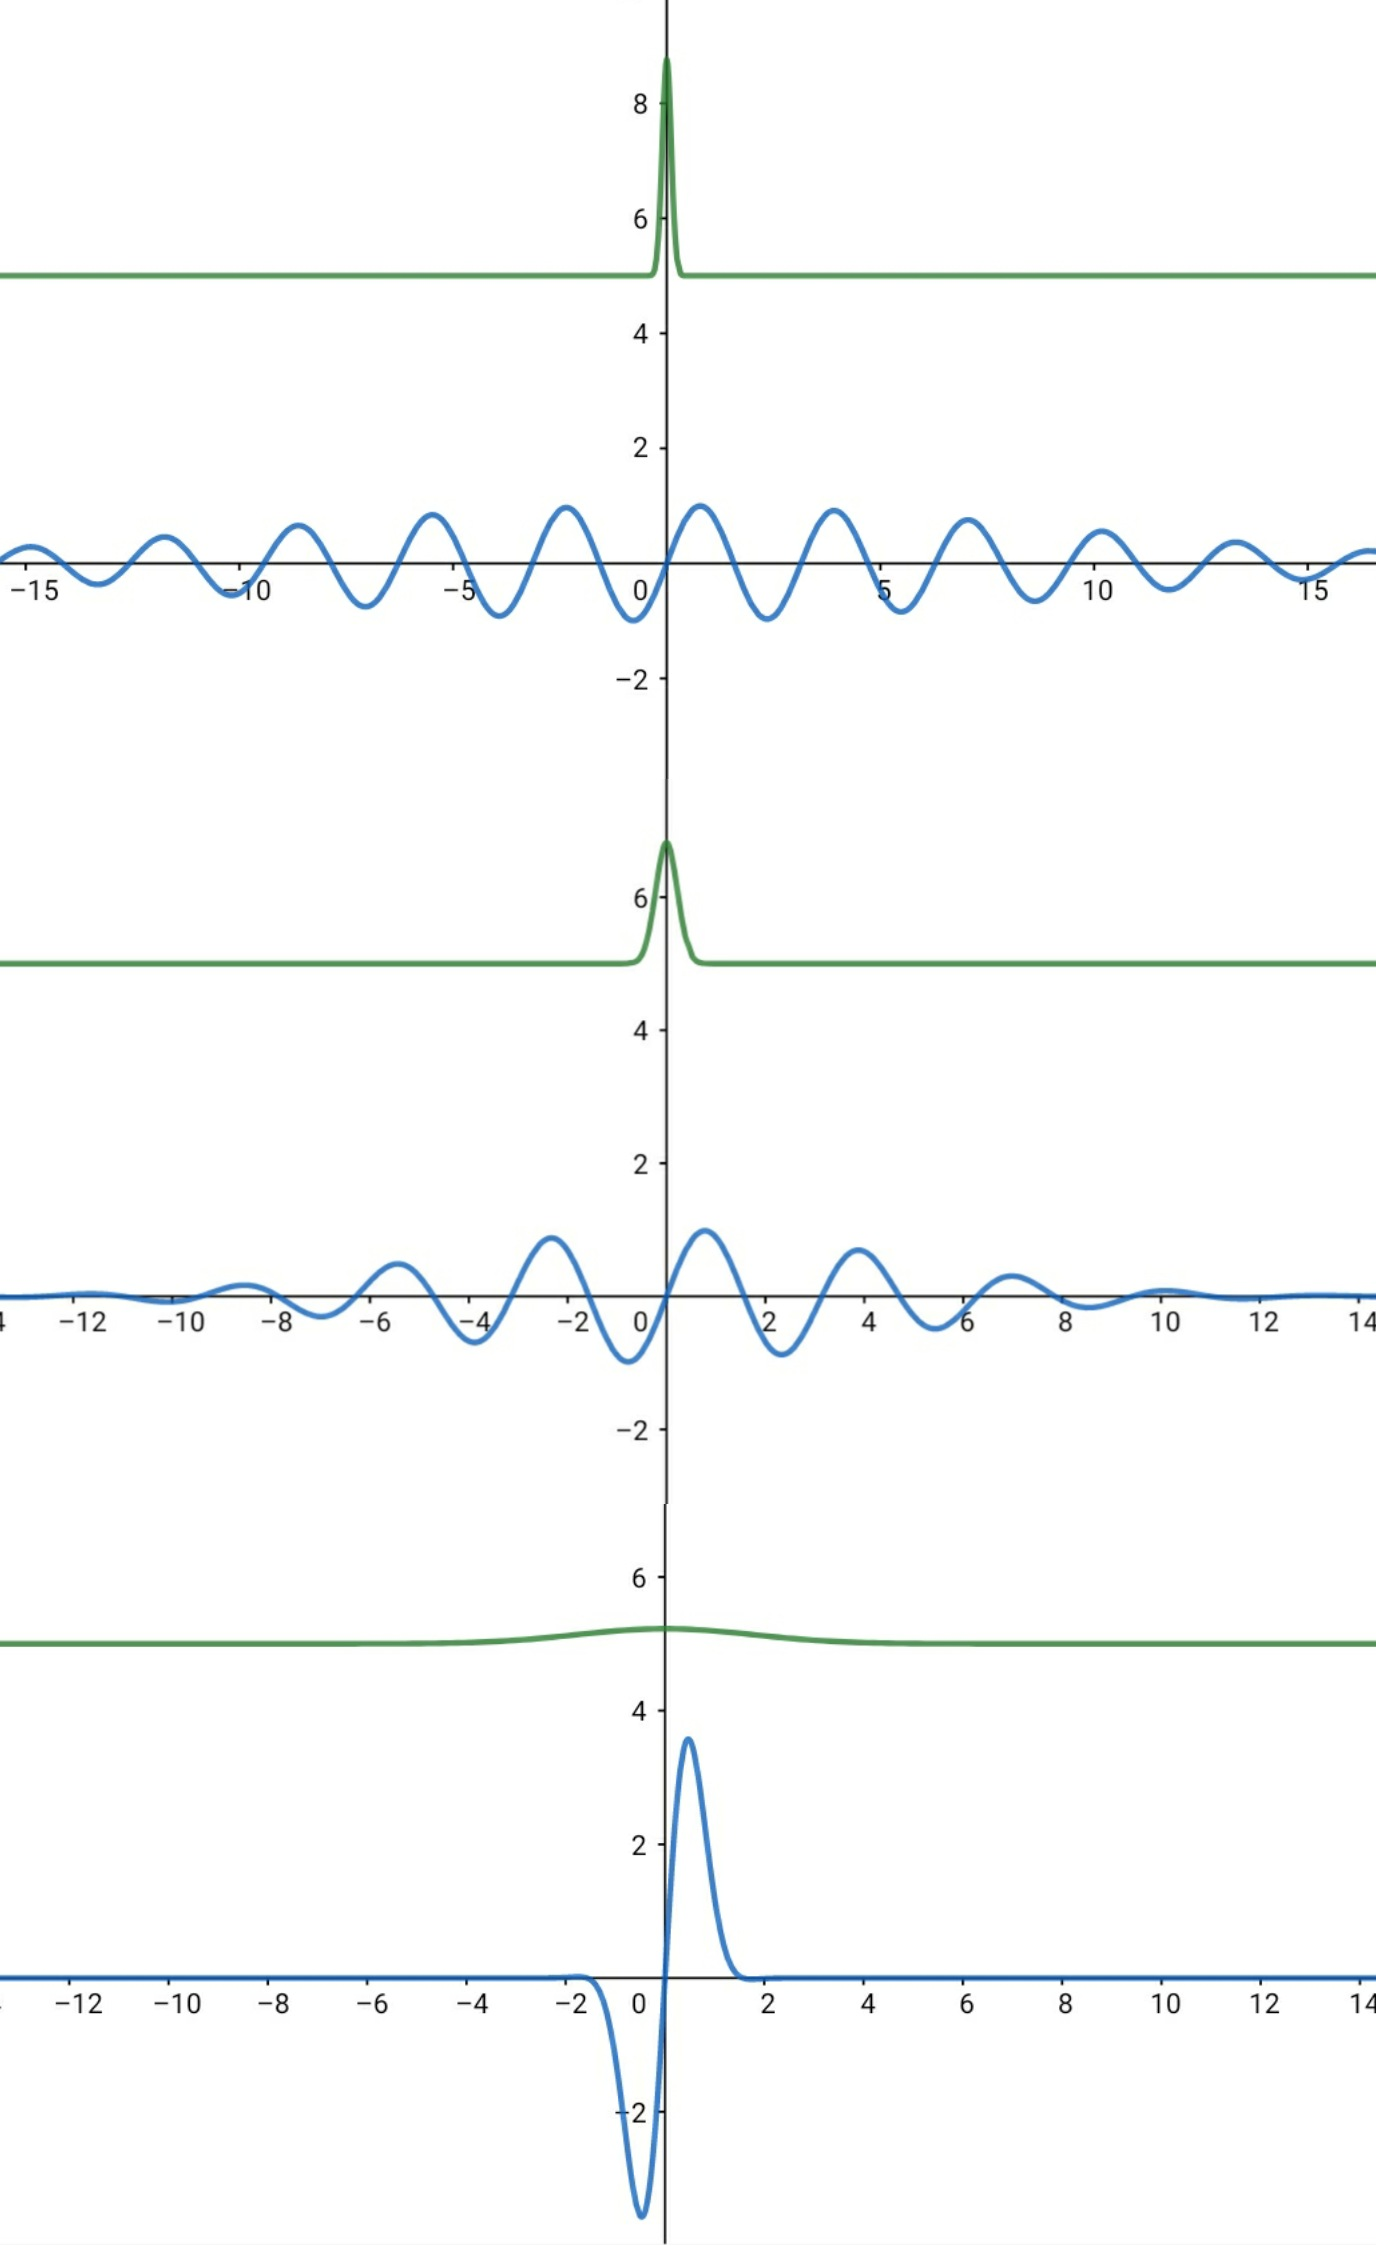
\includegraphics[width=1.3\textwidth]{Im/gausss.jpg}
    \caption{Paquete de ondas (azul) y su respectiva transformada de Fourier (verde), para $\Delta k_x=0.09$, $\Delta k_x=0.34$ y $\Delta k_x=2.54$}
    \label{fig:gau}
\end{marginfigure}
\vspace{0.5cm}

\begin{resultados}{}
Ahora veamos que la relación inversa $\Delta x = \frac{2}{\Delta k_x}$ nos dice que cuanto más ancha es la Gaussiana asociada a $\hat{u}(k_x)$ más angosta será la asociada a $u(x,0)$ y viceversa. Es más, la Gaussiana se hace tan fina hasta llegar a una función delta en el límite cuando $\hat{u}(k_x)=\text{cte}$\\ e inversamente el paquete de ondas se expande a una sola onda plana de ancho infinito cuando $\hat{u}(k_x)$ es una función delta.
\end{resultados}


\vspace{0.5cm}

La relación inversa entre $\Delta x$ y $\Delta k_x$ no es una simple propiedad de la función Gaussiana, así como tampoco es una propiedad del seno la relación inversa entre la frecuencia de la onda $\omega_0$ y el número de ciclos $N$ como en el caso de la sección anterior. Para ver esto con un poco más de detalle consideremos un paquete que se extiende en el intervalo $[x, x+\Delta x]$ compuesto por ondas planas cuyos vectores de propagación se expanden en el intervalo $[k,k+\Delta k]$.Tomemos el siguiente par de ondas: La onda $\mathrm{exp}(ikx)$, la cual sufre un cambio de fase $k\Delta x$ desde el principio hasta el final del paquete. Y la onda  $\mathrm{exp}(i(k+\Delta k)x)$ que sufre un cambio de fase $(k+\Delta k)\Delta x$ a través del paquete.

Veamos en la figura \ref{fig:paquete} como $u(x,0) = u(x+\Delta x,0)= 0$ (ambos extremos del paquete) la diferencia de fase entre las dos ondas 'externas' que nombramos debe ser aproximadamente $2\pi$ para que efectivamente exista interferencia destructiva.
\begin{equation}
    (k+\Delta k)\Delta x - k\Delta x \sim 2 \pi \Rightarrow \Delta x\Delta k \sim 2\pi
    \label{comp}
\end{equation}
Esta última ecuación así como los casos estudiados anteriormente reflejan el concepto de \textbf{complementariedad} entre, en este caso, $\Delta x$ y $\Delta k$. Este concepto es fundamental para estudiar la superposión de ondas planas y en el análisis de Fourier. En el apartado (e) del ejercicio que resolveremos al final se deduce la ecuación \ref{comp} con mucho más detalle mediante el análisis de las \textbf{variancias} de $\hat{u}(k)$ y $u(x)$ y se llega a que las mismas satisfacen:

\begin{equation}\label{desig1}
    \Delta x\Delta k_x \geq \frac{1}{2}
\end{equation}
\begin{marginfigure}
\begin{qbox}{}
   Si recordamos la \textbf{relación de de Broglie}:
   $$\mathbf{p}=\hbar\mathbf{k}$$
   la desigualdad (\ref{desig1}) se transforma en el \textbf{principio de incertibumbre de Heisenberg.}
\end{qbox}

\end{marginfigure}
para el paquete de ondas escalar. Este resultado, como veremos más adelante, constituye un caso particular del \textbf{Principio de Incertidumbre Generalizado}.
 
\newpage
\begin{intro}{}
\textbf{Para demostrar el Principio de Incertidumbre}, necesitamos varias definiciones nuevas. Lo siguiente está extraído de las secciones 1.1 a 1.11 de \textbf{Molecular Quantum Mechanics} (Atkins, Friedman).
\end{intro}

\section{\huge{Introducción a los operadores}}

\textcolor{myred}{\hrule}

\newthought{Un operador es}, en síntesis, un símbolo que contiene instrucciones para llevar a cabo alguna acción sobre una función. Como estamos trabajando con ondas, y las ondas cumplen con el \textbf{principio de superposición}, en particular nos interesará trabajar con \textbf{operadores lineales}. Es decir, un operador $O$ tal que, para las funciones $f$ y $g$, y los escalares $\alpha$ y $\beta$:

\begin{marginfigure}
\begin{qbox}{}
    En mecánica cuántica, los operadores se utilizan para describir observables. En particular, si usamos la \textbf{representación de posición}, el \textbf{operador posición es}:
    \begin{equation*}
        x \longrightarrow x \times
    \end{equation*}
    
    El operador \textbf{momento lineal} es:
    \begin{equation*}
        p_x \longrightarrow \frac{\hbar}{i}\frac{\partial}{\partial x}
    \end{equation*}
    
    Estos operadores actúan sobre funciones $\psi(\mathrm{r},t)$, que son llamadas \textbf{funciones de onda} y caracterizan el \textbf{estado de un sistema}.
\end{qbox}
\end{marginfigure}

\begin{equation}
    O(\alpha\,f+\beta\,g)=\alpha\, O f + \beta\, O g
\end{equation}

\subsection{\textbf{Conmutación y No-conmutación}}

Una característica muy importante de los operadores es que, en general, el resultado de sucesivas operaciones depende del orden en el cual se lleven a cabo. Es decir que, en general $BA\neq AB$, los operadores \textbf{no conmutan}.

Vamos a definir al \textbf{conmutador} de dos operadores $A$ y $B$ de la siguiente manera:

\begin{marginfigure}
\begin{qbox}{}
    El conmutador entre $x$ y $p_x$ es:
    \begin{equation*}
        \left[x,p_x\right]=i\hbar
    \end{equation*}
\end{qbox}
\end{marginfigure}

\begin{equation}\label{conmutdef}
    \left[A,B\right] = AB-BA
\end{equation}
Evidentemente, diremos que dos operadores no conmutan cuando su conmutador sea distinto de 0.
\subsection{\textbf{Notación de Dirac}}

Normalmente vamos a estar trabajando con integrales sobre los operadores y las funciones, es decir, expresiones del tipo (producto interno entre $f$ y $Og$):

\begin{equation}
    I=\int d^3r \, f^*(\mathbf{r)} \,O g(\mathbf{r})
\end{equation}

Como eventualmente vamos a trabajar con muchas integrales de este estilo, es conveniente introducir ahora la notación de Dirac donde el \textbf{bracket} representa\footnote{ También se pueden representar de la siguiente manera: $$ \langle f |\,O\,g \rangle$$ que ayuda a visualizar la idea de producto interno entre el vector fila $ \langle f |$ (bra) y el vector columna $|\,O\,g \rangle$ (ket).} :

\begin{equation}
    \langle f |\,O\,|g \rangle = \int d^3r \, f^*(\mathbf{r)} \,O g(\mathbf{r})
\end{equation}

En particular, podemos escribir:

\begin{equation}
    \langle f |f \rangle = \int d^3r \, f^*(\mathbf{r)}  f(\mathbf{r})
\end{equation}

Que es la \textbf{norma} de una dada función. Evidentemente, si $    \langle f |f \rangle=1$ diremos que una función está \textbf{normalizada}.

En general, vamos a utilizar tanto la notación integral como los brackets de Dirac, para que el cambio de notación no resulte tan agresivo.

\subsection{\textbf{Operadores hermitianos}}

Un \textbf{operador hermitiano} es un operador $O$ que satisface la siguiente relación:

\begin{marginfigure}
\begin{qbox}{}
    Un postulado de la mecánica cuántica dice que \textbf{los observables son representados por operadores hermitianos que satisfacen:}
    \begin{equation*}
    \begin{split}
        \left[q,p_{q'}\right]& = i\hbar \delta_{qq'} \hspace{0.2cm} \left[q,q'\right]=0 \hspace{0.2cm}\\ &\left[p_q,p_{q'}\right]=0
    \end{split}
    \end{equation*}
\end{qbox}
\end{marginfigure}

\begin{equation}
    \int d^3r \, f^*(\mathbf{r)} \,O g(\mathbf{r})=\left(\int d^3r \, g^*(\mathbf{r)} \,O f(\mathbf{r})\right)^*
\end{equation}

O, de modo alternativo, si:

\begin{equation}
    \int d^3r \, f^*(\mathbf{r)} \,O g(\mathbf{r})=\int d^3r \, (O\,g(\mathbf{r)})^* f(\mathbf{r})
\end{equation}

O, en la nueva notación introducida:

\begin{equation}
        \langle f |\,O\,|g \rangle=    \langle g |\,O\,|f \rangle^*
\end{equation}

\subsection{\textbf{Valor esperado}}

El \textbf{valor esperado} de un operador $O$ para una función arbitraria $f$
se nota $\langle O \rangle$, y se define como\footnote{Cuando estemos realizando transformadas de Fourier a las funciones, vamos a introducir un subíndice para explicitar con qué variable estamos trabajando.}:

\begin{marginfigure}
\begin{qbox}{}
    Otro postulado de la mecánica cuántica: para un sistema descripto por una función de onda $\psi$, \textbf{el valor medio de un observable $O$ en una serie de mediciones es igual al valor esperado del operador correspondiente}.
\end{qbox}
\end{marginfigure}
\begin{marginfigure}
\begin{qbox}{}
    Es decir, los operadores 'representan' la posición o el momento, y para calcular su valor esperado hacemos un sanguchito del operador entre $\psi^*$ y $\psi$ e integramos (Griffiths).
\end{qbox}
\end{marginfigure}

\begin{equation}\label{vedef}
    \langle O \rangle =\frac{\int_{-\infty}^{\infty}dx\,f^*(x) \,O f(x)}{\int_{-\infty}^{\infty}dx \,f^*(x) f(x)}= \frac{\langle f |\,O\,|f\rangle}{\langle f|f\rangle}
\end{equation}

Por simplicidad pasamos al caso unidimensional. Observemos además que, si estamos trabajando con funciones normalizadas, la expresión para el valor esperado se reduce a:

\begin{equation}
    \langle O \rangle =\int_{-\infty}^{\infty}dx\,f^*(x) \,O f(x)= \langle f |\,O\,|f\rangle
\end{equation}

\subsection{\textbf{Incertidumbre}}

Para un dado operador (un observable) $O$ podemos definir su 'incertidumbre' (que en realidad se trata de la \textbf{raíz de la desviación cuadrática media}) como sigue:

\begin{equation}\label{incertdef}
    \Delta O=\sqrt{\langle O^2\rangle-\langle O \rangle^2}
\end{equation}

Vamos a definir, además, la \textbf{desviación} de un operador respecto de su valor esperado de la siguiente manera:

\begin{equation}\label{desvdef}
      \delta O = O - \langle O \rangle
\end{equation}
\newpage

\newthought{Ejercicio 16.14 - Zangwill}

\section{\huge{Resolución del ejercicio}}
\textcolor{myred}{\hrule}
\vspace{0.5cm}
\subsection{\textbf{Apartado (a)}}
Sean $f(x)$ y $\hat{f}(x)$ pares de transformaciones de Fourier, entonces
\begin{equation}
    f(x) = \frac{1}{2\pi}\int_{-\infty}^{\infty} dk \hat{f}(k) e^{ikx}
    \label{trans}
\end{equation}
\begin{equation}
    \hat{f}(k) = \int_{-\infty}^{\infty} dx f(x) e^{-ikx}
    \label{antitrans}
\end{equation}

Ahora sea $h(x)=f'(x)$, entonces su antitransformada de Fourier será
\begin{equation}
    \hat{h}(k) = \int_{-\infty}^{\infty} dx h(x) e^{-ikx} = \int_{-\infty}^{\infty} dx f'(x) e^{-ikx}
\end{equation}
integramos por partes la ecuación anterior y obtenemos 
\begin{equation}
        \int_{-\infty}^{\infty} dx f'(x) e^{-ikx} =  e^{-ikx} f(x) \biggr|_{-\infty}^{\infty} - \int_{-\infty}^{\infty} dx f(x) (-ik)e^{-ikx} 
\end{equation}
dado que $f(x)$ se anula\footnote{$f(x)$ debe anularse cuando $x \to \pm \infty$ para que la transformada de Fourier de $f(x)$ exista.} cuando $x \to \pm \infty$ tenemos
\begin{equation}
    \hat{h}(k) = ik ~\underbrace{\int_{-\infty}^{\infty} dx f(x) e^{-ikx}}_{ \hat{f}(k)}
\end{equation}
donde aplicamos ec.\ref{antitrans}, y llegamos a la relación pedida
\begin{equation}
    \hat{h}(k) = ik \hat{f}(k)
\end{equation}

\subsection{\textbf{Apartado (b)}}
Queremos probar la siguiente relación
\begin{equation}
    \frac{1}{2\pi}~ \int_{-\infty}^{\infty} dk \hat{f^*}(k) g(k) = \int_{-\infty}^{\infty} dx f^*(x) g(x)
    \label{parseval}
\end{equation}

Comenzaremos reemplazando en el lado derecho las funciones $f^*(x)$ y $g(x)$ por sus antitransformadas

\begin{equation}
\int_{-\infty}^{\infty} dx f^*(x) g(x) = \int_{-\infty}^{\infty} \frac{1}{2\pi} \int_{-\infty}^{\infty} dk'~\hat{f^*}(k') e^{-ik'x} ~\frac{1}{2\pi} \int_{-\infty}^{\infty} dk~\hat{g}(k) e^{ikx} ~~dx \overset{\dagger}{=}
\end{equation}
donde hemos aplicado la propiedad de la transformada de la conjugada de una función y entonces reordenando 
\begin{equation}
\overset{\dagger}{=} \int_{-\infty}^{\infty}  \frac{1}{2\pi} \int_{-\infty}^{\infty} \hat{f^*}(k') \hat{g}(k) ~\underbrace{\frac{1}{2\pi}  \int_{-\infty}^{\infty} e^{ix(k-k')}~ dx}_{\delta(k-k')} dk dk' \overset{\dagger}{=}
\end{equation}

El término señalado en la última igualdad corresponde a una representación de la función delta de Dirac\cite[][Sec. 15.2]{arfken} y luego
\begin{equation}
\overset{\dagger}{=}\frac{1}{2\pi} \int_{-\infty}^{\infty} \hat{f^*}(k') \underbrace{\int_{-\infty}^{\infty} \hat{g}(k) \delta(k-k')~ dk}_{\hat{g}(k')} dk' = \frac{1}{2\pi} \int_{-\infty}^{\infty} \hat{f}(k') \hat{g}(k') dk'
\end{equation}
donde hemos aplicado la definición de la delta de Dirac.

Finalmente hemos llegado al lado izquierdo de la relación \ref{parseval} y por lo tanto queda demostrado el \textbf{teorema de Parseval}.



\subsection{\textbf{Apartado (c)}}

En este apartado, se nos pide demostrar que:

\begin{equation}\label{enun.c}
    \langle k \rangle_k=-i\langle\frac{d}{dx}\rangle
    _x\hspace{0.7cm} \text{y} \hspace{0.7cm} \langle k^2 \rangle_k=-\langle \frac{d^2}{dx^2}\rangle_x
\end{equation}

Comencemos por el primero. Recordemos que, por definición, el \textbf{valor esperado} $\langle k \rangle_k$ es:

\begin{equation}\label{int.c}
    \langle k \rangle_k= \frac{\langle \hat{f} |\,k\,|\hat{f}\rangle}{\langle \hat{f}|\hat{f}\rangle}=\frac{\int_{-\infty}^{\infty}dk\,\hat{f}^*(k) k \hat{f}(k)}{\int_{-\infty}^{\infty}dk \,\hat{f}^*(k) \hat{f}(k)}
\end{equation}

Si aplicamos el \textbf{teorema de Parseval} demostrado en el apartado anterior al denominador de esta última expresión, domando $f(x)=g(x)=f(x)$, tenemos que:

\begin{equation}\label{den.c}
    \int_{-\infty}^{\infty}dk \,\hat{f}^*(k) \hat{f}(k)=2\pi \int_{-\infty}^{\infty}dx \,f^*(x) f(k)=2\pi\langle f^*|f\rangle
\end{equation}

Ahora analicemos el numerador de (\ref{int.c}):

\begin{equation}\label{kf.c}
    \int_{-\infty}^{\infty}dk\,\hat{f}^*(k)\left[ k \hat{f}(k)\right]
\end{equation}

Utilizando la propiedad demostrada en el primer apartado, vemos que tomando $h(x)=df/dx$, la expresión entre corchetes es igual a:

\begin{equation}
     k \hat{f}(k)=\frac{1}{i}\hat{h}(k)
\end{equation}

Entonces:

\begin{equation}
    \int_{-\infty}^{\infty}dk\,\hat{f}^*(k)\left[ k \hat{f}(k)\right]=\frac{1}{i} \int_{-\infty}^{\infty}dk\,\hat{f}^*(k)\hat{h}(k)
\end{equation}

Volvemos a utilizar el teorema de Parseval, esta vez tomando $f(x)=f(x)$ y $g(x)=h(x)$:

\begin{equation}
    \frac{1}{i} \int_{-\infty}^{\infty}dk\,\hat{f}^*(k)\hat{h}(k)=\frac{2\pi}{i}\int_{-\infty}^{\infty}dx\,f^*(x)h(x)
\end{equation}

Ahora, si reescribimos a $h(x)$ como el operador $d/dx$ actuando sobre la función $f(x)$, tenemos que:

\begin{equation}\label{num.c}
   \frac{2\pi}{i}\int_{-\infty}^{\infty}dx\,f^*(x) \left(\frac{d}{dx}\right) f(x)=\frac{2\pi}{i}\langle f|\,\frac{d}{dx}\,|f\rangle
\end{equation}

Finalmente, dividiendo las expresiones (\ref{num.c}) y (\ref{den.c}), vemos que los $2\pi$ se cancelan y, si reescribimos $1/i=-i$, llegamos a:

\begin{equation}
    \langle k \rangle_k = -i \frac{\langle f|\,\frac{d}{dx}\,|f\rangle}{\langle f|f\rangle}=\langle \frac{d}{dx}\rangle_x
\end{equation}

Que es exactamente a donde queríamos llegar.

Probar la segunda igualdad de (\ref{enun.c}) es bastante análogo. Veamos:

\begin{equation}\label{int.c2}
    \langle k^2 \rangle_k= \frac{\langle \hat{f} |\,k^2\,|\hat{f}\rangle}{\langle \hat{f}|\hat{f}\rangle}=\frac{\int_{-\infty}^{\infty}dk\,\hat{f}^*(k) k^2 \hat{f}(k)}{\int_{-\infty}^{\infty}dk \,\hat{f}^*(k) \hat{f}(k)}
\end{equation}

La parte de los denominadores es exactamente la misma. La única diferencia es que ahora, en el término entre corchetes de (\ref{kf.c}), tendríamos $k^2 \hat{f}(k)$. Si llamamos $g(x)=dh/dx$ y usamos nuevamente el resultado del apartado (a), tenemos que:

\begin{equation}
    k^2 \hat{f}(k)=k(k\,\hat{f}(k))=\frac{1}{i}k\,\hat{h}(k)=-\hat{g}(k)
\end{equation}

Si ahora usamos el teorema de Parseval para el numerador de (\ref{int.c2}), y luego reconocemos a $g(x)$ como el operador $d^2/dx^2$ actuando sobre la función $f(x)$, tenemos entonces que:

\begin{equation}
     \langle k^2 \rangle_k =-\frac{\langle f|\,\frac{d^2}{dx^2}\,|f\rangle}{\langle f|f\rangle}=-\langle \frac{d^2}{dx^2}\rangle_x
\end{equation}


\subsection{\textbf{Apartado (d)}}

En este apartado se nos pide, utilizando las definiciónes de 'incertidumbre' $\Delta O$ (ecuación \ref{incertdef}), valor esperado (ecuación \ref{vedef} y conmutador (ecuación \ref{conmutdef}) que, para dos operadores hermitianos $A$ y $B$, vale que:

\begin{equation}
    \Delta A \Delta B \geq \frac{1}{2}\left| i \langle \left[A,B\right]\rangle_x\right|
\end{equation}

Es decir, queremos demostrar el \textbf{principio de incertidumbre generalizado}\cite[][p.27]{atkins}. Let's do it.

Vamos a suponer, primero, que los operadores $A$ y $B$ son tales que su conmutador satisface:

\begin{equation}
    \left[A,B\right]=i C
\end{equation}

También vamos a suponer que ambos operadores actúan sobre una misma función $f(x)$, que por simplicidad la supondremos normalizada, de modo tal que:

\begin{equation}
    \langle A \rangle_x = \int_{-\infty}^{\infty}dx\,f^*(x) A f(x)=\langle f|A|f\rangle 
\end{equation}

Y análogamente

\begin{equation}
    \langle B \rangle_x = \int_{-\infty}^{\infty}dx\,f^*(x) B f(x)=\langle f|B|f\rangle 
\end{equation}

Recordemos que, tal como los definimos en la ecuación (\ref{desvdef}), las \textbf{desviaciones} de $A$ y $B$ respecto de sus valores esperados son;

\begin{equation}
    \delta A = A - \langle A \rangle_x \hspace{0.7cm} y \hspace{0.7cm} \delta B = B - \langle B \rangle_x
\end{equation}

Ahora calculemos el conmutador de $\delta A$ y $\delta B$. Recordemos que los valores esperados $\langle A \rangle$ y $\langle B \rangle$ son números\footnote{Abandonamos los subíndices para simplificar la notación y porque la única variable presente es $x.$} (no son operadores) y sí pueden conmutarse entre sí y con los operadores:

\begin{equation}
    \begin{split}
   \left[\delta A, \delta B \right] &= \left[A - \langle A \rangle , B - \langle B \rangle \right]= \\
   &=AB-A\langle B \rangle - \langle A \rangle B + \langle A \rangle\langle B \rangle\\
   &-BA+B\langle A \rangle+\langle B \rangle A-\langle B \rangle\langle A \rangle = \left[A,B\right]=iC\\
    \end{split}
\end{equation}

Ahora consideremos la siguiente integral, donde $\alpha$ es una constante real arbitraria:

\begin{equation}
    I= \int_{-\infty}^{\infty}dx |(\alpha \, \delta A - i \,\delta B)f(x)|^2
\end{equation}

El integrando es claramente positivo para todo $x$, por lo que la integral será no-negativa. Podemos desarrollar esta integral como:

\begin{equation}
    I= \int_{-\infty}^{\infty}dx \{(\alpha \, \delta A - i \,\delta B)f(x)\}^*\{(\alpha \, \delta A - i \,\delta B)f(x)\}
\end{equation}

Como los operadores son hermitianos, si tomamos $g(x)$ como el término entre los primeros cochetes, $O=(\alpha \, \delta A - i \,\delta B)$ y $f(x)=f(x)$, podemos reescribir la integral como:

\begin{equation}
    I=\int_{-\infty}^{\infty}dx f^*(x)(\alpha \, \delta A + i \,\delta B)(\alpha \, \delta A - i \,\delta B)f(x)
\end{equation}

Esta última expresión tiene a su vez la forma un valor esperado, entonces:

\begin{equation}
    I=\langle (\alpha\,\delta A + i\,\delta B)(\alpha\,\delta A - i\,\delta B)\rangle
\end{equation}

Expandiendo los productos y aplicando la linealidad de los valores esperados:

\begin{equation}
    I=\alpha^2\langle(\delta A)^2\rangle + \langle(\delta B)^2\rangle- i\alpha \underbrace{\langle \delta A\delta B - \delta B \delta A \rangle}_{=\langle\left[\delta A, \delta B\right]\rangle=\langle i C\rangle}
\end{equation}

Entonces tenemos que:

\begin{equation}
    I= \alpha^2\langle(\delta A)^2\rangle + \langle(\delta B)^2\rangle +\alpha \langle C \rangle
\end{equation}

Esto tiene la forma de una expresión cuadrática en $\alpha$. Si completamos cuadrados, podemos reescribirla como:

\begin{equation}\label{int.i}
    I=\langle(\delta A)^2\rangle \left( \alpha + \frac{\langle C \rangle}{2\langle(\delta A)^2\rangle}\right)^2+\langle(\delta B)^2\rangle - \frac{\langle C \rangle^2}{4\langle(\delta A)^2\rangle}
\end{equation}

Ahora bien, habíamos dicho que $I$ debe ser no-negativa para cualquier valor de $\alpha$. En particular, seguirá siendo no negativa cuando elijamos en valor de $\alpha$ donde $I$ alcanza su mínimo. Como el primer término de (\ref{int.i}) siempre aporta una contribución positiva a $I$, este valor de $\alpha$ será tal que la expresión entre paréntesis sea nula. Para ese $\alpha$, tenemos\footnote{Un argumento más directo para esto es utilizar la desigualdad de Cauchy-Schwartz, sin embargo optamos por esta demostración para no agregar más contenido teórico al trabajo.}:

\begin{equation}
    I=\langle(\delta B)^2\rangle-\frac{\langle C \rangle^2}{4\langle(\delta A)^2\rangle}\geq 0
\end{equation}

Entonces:

\begin{equation}
    \langle(\delta A)^2\rangle\langle(\delta B)^2\rangle\geq \frac{1}{4}\langle C \rangle^2
\end{equation}

Ahora, veamos que los valores esperados de la izquierda puede reescribirse como sigue:

\begin{equation}
\begin{split}
     \langle(\delta A)^2\rangle &=\langle(A- \langle A\rangle)^2\rangle=\langle A^2 - 2 A \langle A \rangle + \langle A \rangle^2 \rangle   \\ 
     &= \langle A^2\rangle - 2\langle A\rangle\langle A\rangle+ \langle A\rangle^2 = \langle A^2\rangle -\langle A\rangle^2=(\Delta A)^2
\end{split}
\end{equation}

El desarrollo para $B$ es idéntico, y entonces la desigualdad se transforma en:

\begin{equation}
    \Delta A \Delta B \geq \frac{1}{2}|\langle C \rangle|
\end{equation}

Recordando que $\left[A,B\right]=iC$, podemos reemplazar y obtenemos:

\begin{equation}
     \Delta A \Delta B \geq \frac{1}{2}|\langle i \left[A,B\right] \rangle|
\end{equation}

Que es exactamente a lo que queríamos llegar.\footnote{Decidimos dejar la unidad imaginaria $i$ multiplicando puesto que, además de ser la expresión que aparece en el enunciado, también nos recuerda que la expresión dentro de las barras de módulo es real, puesto que el conmutador entre dos operadores hermitianos es \textbf{anti-hermitiano}, y su valor esperado es imaginario. La $i$ que aparece explícitamente cancela la $i$ propia de $\left[A,B\right]$}.

\subsection{\textbf{Apartado (e)}}

Ahora, vamos a utilizar todo lo desarrollado anteriormente para demostrar que, si $\Delta k =\sqrt{\langle k^2 \rangle_k-\langle k\rangle^2_k}$, se cumple que:

\begin{equation}
    \Delta x \Delta k \geq \frac{1}{2}
\end{equation}

Vamos, primero, a reemplazar los valores esperados $\langle k^2\rangle $ y $\langle k \rangle ^2$ según lo demostrado en el apartado (c) en $\Delta k$. Tenemos:

\begin{equation}
    \begin{split}
        \Delta k &= \sqrt{-\langle \frac{d^2}{dx^2} \rangle_x-\left(-i\langle \frac{d}{dx}\rangle_x\right)^2}\\
        &=\sqrt{\langle -\left( \frac{d}{dx}\right)^2 \rangle_x-\left(-i\langle \frac{d}{dx}\rangle_x\right)^2}\\
        &=\sqrt{\langle \left(-i\frac{d}{dx}\right)^2 \rangle_x-\left(\langle -i\left(\frac{d}{dx}\right)\rangle_x\right)^2}=\Delta\left(-i\frac{d}{dx}\right)
    \end{split}
\end{equation}

Ahora, aplicamos el principio de incertidumbre ya demostrado, usando $A=x$ y $B=-i(d/dx)$. Veamos:

\begin{equation}
     \Delta x \Delta k =  \Delta x \Delta \left(-i\frac{d}{dx}\right) \geq \frac{1}{2}|\langle i \left[x,-i\frac{d}{dx}\right]\rangle_x|
\end{equation}

Tenemos que calcular el conmutador $\left[x,-i\frac{d}{dx}\right]$. Para ello, supongamos que estamos operando sobre una función genérica $f(x)$:

\begin{equation}
 \begin{split}
    \left[x,-i\frac{d}{dx}\right]f&=\left(-ix\frac{d}{dx}+i\frac{d}{dx}x\right)f\\
    &=-ix\frac{df}{dx}+i\frac{d(xf)}{dx}= -ix\frac{df}{dx}+ix\frac{d(f)}{dx}+if\frac{dx}{dx}=if     
 \end{split}
\end{equation}

Tenemos entonces que el conmutador es igual a $i$. Entonces:

\begin{equation}
     \Delta x \Delta k \geq \frac{1}{2}|\langle i \cdot i \rangle|=\frac{1}{2} 
\end{equation}

\begin{marginfigure}
\begin{qbox}{}
    Recordemos que, para los operadores posición y momento lineal, su conmutador era igual a $i\hbar$. Esto quiere decir que:
    \begin{equation*}
    \Delta x \Delta p_x \geq \frac{1}{2}|\langle i \cdot i \hbar \rangle| = \frac{\hbar}{2}
    \end{equation*}
\end{qbox}
\end{marginfigure}

Que es a donde queríamos llegar.

Como podemos ver, hay un 'principio de incertidumbre' para cada par de observables cuyos operadores no conmuten, los cuales de denominan \textbf{operadores incompatibles}.

\vspace{0.5cm}
\begin{resultados}{}
    El principio de incertidumbre no es una suposición de la teoría cuántica, sino que es una \textbf{consecuencia de la interpretación estadística}.
\end{resultados}
\begin{resultados}{}
Al medir, por ejemplo, la posición $x$ de una partícula, la acción de medirla colapsa a la función de onda en un pico delgado, \textbf{cuya descomposición de Fourier} tiene, en consecuencia, un amplio rango de longitudes de onda (y por lo tanto momentos lineales $p_x$).
Existe, de hecho, un 'principio de incertidumbre' para \textbf{todo par de observables cuyos operadores no conmuten}, y los llamamos \textbf{observables incompatibles}.   
\end{resultados}
\begin{resultados}
Si, por otro lado, medimos el momento $p_x$, el estado colapsa a una onda sinusoidal larga, con longitud de onda bien definida, pero la partícula ya no tiene la posición de la medición anterior.
\end{resultados}
